\chapter{Detectability in next-generation galaxy surveys}
\label{chapter:detect}


In this chapter, we investigate whether the next generation of high-precision cosmological surveys will be able to make such a detection. First, we consider a Stage IV spectroscopic $H\alpha$ survey similar to Euclid, and we find that the cumulative signal to noise of this relativistic signature  is $\ord(10)$. Secondly, we look at some future 21cm intensity mapping surveys; MeerKAT, SKA, PUMA, and HIRAX. Due to foreground and telescope beam effects, the signal-to-noise ratio for intensity mapping surveys is typically lower than for spectroscopic $H\alpha$ surveys, though also still detectable.

\section{Detecting the leading-order relativistic signature}


Here we highlight a feature of the tree-level Fourier galaxy bispectrum which follows from the  leading-order relativistic contribution -- due to Doppler, gravitational redshift  and related line-of-sight effects -- that is omitted in the standard Newtonian analysis. These effects generate an imaginary part of the galaxy bispectrum, which can be understood as follows (see also \cite{McDonald:2009dh,Clarkson:2018dwn,Jeong:2019igb} for a more general discussion).  
The Doppler-type contributions to the galaxy density contrast involve one or three derivatives  of scalars along the fixed line of sight $\bm n$ [see \eqref{dg1}, \eqref{eq:dgsecond} below]. In Fourier space, with the plane-parallel approximation, we have  $\bm{n}\cdot\bm{\nabla} \to {\i}\, \bm{n}\cdot\bm{k}$, and this leads to imaginary corrections to the galaxy density contrast, which do not cancel in the bispectrum, unlike in the power spectrum. At first order, we have $\delta_g=\delta_{g\mathrm{N}}+ \delta_{g\mathrm{D}}$, where the Newtonian part $\delta_{g\mathrm{N}}$ is real and scales as the linear matter density contrast $\delta$. The 
relativistic Doppler-type part $\delta_{g\mathrm{D}}$ scales as ${\i}\,(\cH/k) \delta$  (see \cite{McDonald:2009dh, Jeong:2011as, Abramo:2017xnp,Clarkson:2018dwn} and below). At second  order, the relativistic contribution $\delta_{g\mathrm{D}}^{(2)}$ scales as ${\i}\,(\cH/k) (\delta)^2$ (see \cite{Clarkson:2018dwn} and below). 


In the case of  the galaxy {auto}-power spectrum, $P_g\sim \langle |\delta_g|^2\rangle$, the relativistic part is {real and scales as} $(\cH/k)^2P$\,:  therefore we can neglect $P_{g\mathrm{D}}$ at leading order. By contrast, for the galaxy bispectrum, $B_g\sim \langle \delta_g\,\delta_g \, \delta^{(2)}_g\rangle$, a coupling of relativistic contributions to short-scale Newtonian terms (which  is absent in $P_g$) produces a $B_{g\mathrm{D}}$ that is {imaginary and scales as} ${\i}\,(\cH/k)P^2$. 
We therefore expect these relativistic effects to be more accessible in the bispectrum than in the power spectrum, for the case of a single tracer {of the matter distribution}. \todo{leave some points about relativistic effects detect. in P vs B}

Although the galaxy bispectrum is statistically isotropic, the plane-parallel approximation in redshift space breaks 3-dimensional isotropy, since a preferred direction is imposed by the observer's fixed line of sight. 

Let us introduce a more explicit analysis, as follows.

At tree-level, the Fourier galaxy bispectrum at  a redshift $z$ is given by
\begin{equation}
{\big\langle \delta_g(z,\bm{k}_{1})\delta_g(z,\bm{k}_{2})\delta^{(2)}_g(z,\bm{k}_{3}) \big\rangle + \text{2 cp}=2 (2\pi)^3 B_{g}(z, \bm{k}_{1}, \bm{k}_{2}, \bm{k}_{3}) \delta^{\mathrm{Dirac}}\big(\bm{k}_{1}+ \bm{k}_{2}+ \bm{k}_{3} \big)\,,}
\end{equation}
where cp denotes cyclic permutation and the factor 2 on the right arises from the convention that the total number density contrast is $\delta_g+ \delta^{(2)}_g/2$.  
In terms of the first- and second-order kernels, we have
\begin{equation}
B_{g}(z, \bm{k}_{1}, \bm{k}_{2}, \bm{k}_{3}) = \mathcal{K}^{(1)}(z, \bm{k}_{1})\mathcal{K}^{(1)}(z, \bm{k}_{2})\mathcal{K}^{(2)}(z, \bm{k}_{1}, \bm{k}_{2}, \bm{k}_{3})P(z, k_{1})P(z, k_{2}) + \text{2 cp}\,, \label{eq:bkern}
\end{equation}
where $P$ is the linear matter power spectrum. 
The $9-3=6$ degrees of freedom in the triangle condition $\bm{k}_{1}+ \bm{k}_{2}+ \bm{k}_{3}=\bm{0}$ at each $z$ are reduced to 5 by the fixed observer's line of sight direction $\bm{n}$.
The bispectrum can be chosen at each $z$ to be a function  of the 3 magnitudes ${k_a}=\big({k}_{1}, {k}_{2},{k}_{3}\big)$ and 2 angles that define the orientation of the triangle (see Fig. \ref{fig0}):
\begin{equation}
B_{g}(z, \bm{k}_{a}) =B_{g}(z, {k}_{a},  \mu_1,\varphi) \,.
\end{equation}
Here $\mu_a=\hat{\bm{k}}_a\cdot\bm{n}=\cos\theta_a$,  and $\varphi$ is the angle between the triangle plane and the $(\bm{n},\bm{k}_1)$-plane. The three angles $\theta_{ab}= \cos^{-1}\big(\hat{\bm{k}}_{a} \cdot \hat{\bm{k}}_b\big)$, are determined by $k_a$; then $\mu_2=\mu_1\cos\theta_{12}+ \sin\theta_1\,\sin\theta_{12}\cos\varphi$ is determined when $\varphi$ is given, and $\mu_3=-(\mu_1k_1+\mu_2k_2)/k_3$.
\begin{figure}[ht]
\centering
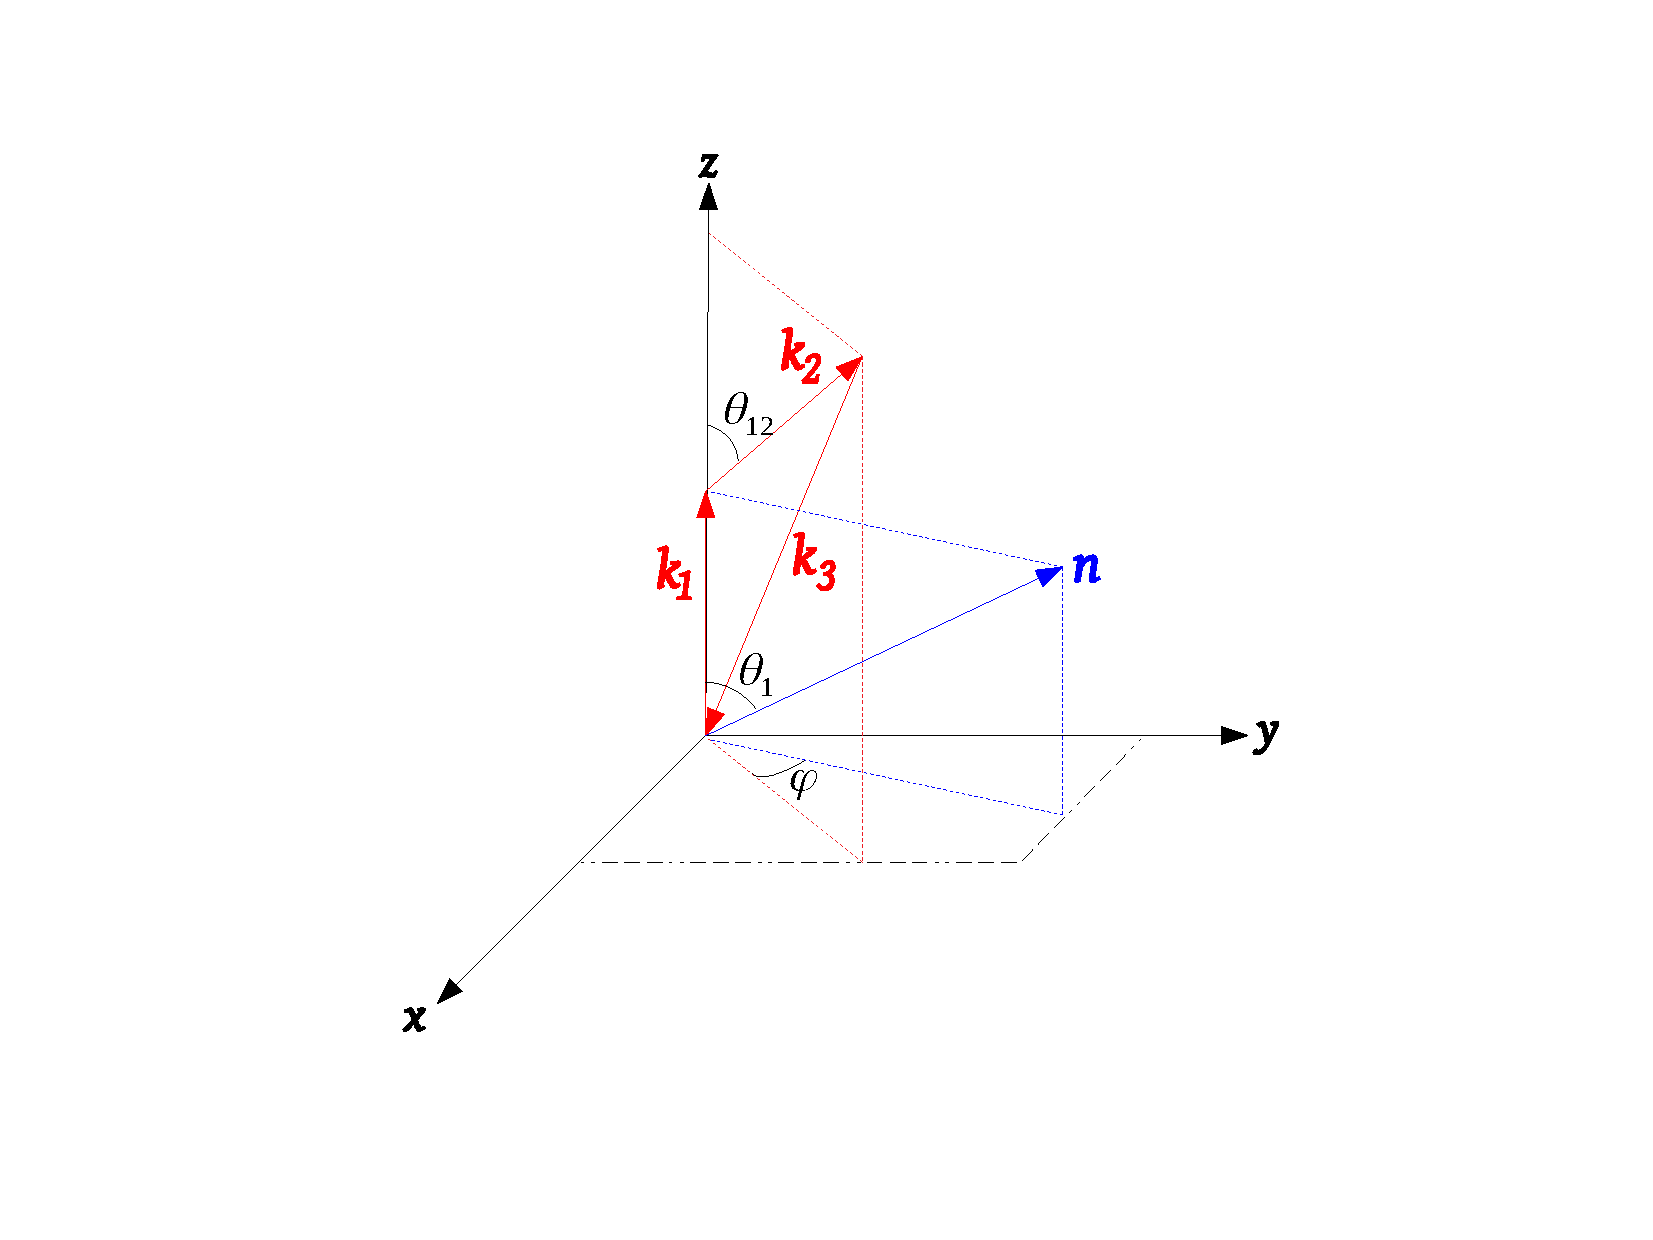
\includegraphics[width=10.0cm]{fig/geometryAngles}
\vspace*{-1cm}
\caption{Relevant vectors and angles for the Fourier bispectrum.} \label{fig0}
\end{figure}

In the standard Newtonian approximation, $B_g=B_{g{\mathrm{N}}}$, the kernels in \eqref{eq:bkern} contain the galaxy bias and the redshift-space distortions (RSD) at first and second order \cite{Bernardeau:2001qr, Karagiannis:2018jdt}:
\begin{align}
\mathcal{K}^{(1)}_{\mathrm{N}}(\bm{k}_{1}) &= b_{1}+f\mu_{1}^{2}\,,  \label{e15} \\ 
{\mathcal{K}^{(2)}_{\mathrm{N}}}(\bm{k}_{1}, \bm{k}_{2},{\bm{k}_3}) &= b_{1}F_{2}(\bm{k}_{1}, \bm{k}_{2}) + b_{2} + f\mu_{3}^{2}G_{2}(\bm{k}_{1}, \bm{k}_{2}) +{fZ_2}(\bm{k}_{1}, \bm{k}_{2})
+ b_{s^{2}}S_{2}(\bm{k}_{1}, \bm{k}_{2}) , \label{k2n}
\end{align}
where we dropped the $z$-dependence for brevity. Here $f$ is the linear matter growth rate, $b_1,b_2$ are the linear and second-order clustering biases, and $b_{s^{2}}$ is the tidal bias. The kernel  $F_2$ is for second-order density, $G_2 , \mathcal{Z}_2$ are for RSD,  and $S_2$  is the kernel for tidal bias (see Appendix~\ref{app_euclid} for the full expressions).


The Doppler-type relativistic corrections to the Newtonian number count contrast in redshift space are  given {at first order by~\cite{Bonvin:2011bg}:}
\begin{equation}
\delta_{g\mathrm{D}} =  {A}\,\bm{v}\cdot\bm{n}\,,\label{dg1}
\end{equation}
{where $A(z)$ is given below in~\eqref{e25} and the momentum conservation equation has been used to  eliminate the gravitational redshift: $\bm{n}\cdot\bm{\nabla}\Phi\equiv \p_r \Phi = -\bm{v}'\!\cdot\bm{n}-\cH\,\bm{v}\cdot\bm{n} $.} Here $\Phi$ is the gravitational potential, $\bm{v}$ is the peculiar velocity,  $\cH$ is the comoving Hubble parameter, and $r$ is the line-of-sight comoving distance.
Note that $\bm{v}\cdot\bm{n}=\partial_r V$, where $V$ is the velocity potential ($v_i=\partial_iV$). 
At second order, and neglecting vector and tensor modes, it is shown in~\cite{Clarkson:2018dwn}  that (see also \cite{DiDio:2018zmk}) 
\begin{align}
\delta^{(2)}_{g{\mathrm{D}}}&= A\, \bm{v}^{(2)}\!\!\cdot\bm{n}+2{C}(\bm{v}\cdot\bm{n})\,\delta +2 \frac{{E}}{\cH}(\bm{v}\cdot\bm{n})\,\partial_r(\bm{v}\cdot\bm{n})
+ \frac{2}{\cH^2}\big[(\bm{v}\cdot\bm{n}) \,\partial_r^2\Phi-\Phi\, \partial_r^2 (\bm{v}\cdot\bm{n}) \big]
\nonumber\\ \label{eq:dgsecond}
& - \frac{2}{\cH}\,\partial_r (\bm{v}\cdot\bm{v}) + 2 \frac{b_1}{\cH}\,\Phi\, \partial_r\delta \,. 
\end{align}
The redshift-dependent coefficients $C,E$ are  given below  in \eqref{e26}, \eqref{e27}.


In Fourier space, 
neglecting sub-leading $ \mathcal{O}(\cH^2/k^2)$ terms, we find from \eqref{eq:bkern} that
\begin{align}
 B_{g\mathrm{D}}(\bm{k}_{1},\bm{k}_{2},\bm{k}_{3}) &=  \bigg\{\bigg[\mathcal{K}^{(1)}_{\mathrm{N}}(\bm{k}_{1})\mathcal{K}^{(1)}_{\mathrm{D}}(\bm{k}_{2}) + \mathcal{K}^{(1)}_{\mathrm{D}}(\bm{k}_{1})\mathcal{K}^{(1)}_{\mathrm{N}}(\bm{k}_{2})\bigg]\mathcal{K}^{(2)}_{\mathrm{N}}(\bm{k}_{1},\bm{k}_{2},\bm{k}_{3}) 
\nonumber \\&  \quad 
+\mathcal{K}^{(1)}_{\mathrm{N}}(\bm{k}_{1})\mathcal{K}^{(1)}_{\mathrm{N}}(\bm{k}_{2})\mathcal{K}^{(2)}_{\mathrm{D}}(\bm{k}_{1},\bm{k}_{2},\bm{k}_{3})\bigg\}P(k_{1})P(k_{2})+\text{2 cp}. \label{e21}
\end{align}
The relativistic kernels follow from \eqref{dg1} and \eqref{eq:dgsecond}; they are given in \cite{Clarkson:2018dwn} as
\begin{align}
\mathcal{K}^{(1)}_{\mathrm{D}}(\bm{k}_{1}) &= \mathrm{i}\,\cH f A\,\frac{\mu_{1}}{k_{1}}\,, \label{e23} \\
\mathcal{K}^{(2)}_{\mathrm{D}}(\bm{k}_{1},\bm{k}_{2},\bm{k}_{3}) &= \mathrm{i}\,\cH f \bigg[
A\,\frac{\mu_{3}}{k_{3}}G_{2}(\bm{k}_{1},\bm{k}_{2})
+C\left(\frac{\mu_{1}}{k_{1}} + \frac{\mu_{2}}{k_{2}}\right)
 +\left(\frac{3}{2}\Omega_{m}-fE\right)\mu_{1}\mu_{2}\left(\frac{\mu_{1}}{k_{2}}+\frac{\mu_{2}}{k_{1}}\right)
\nonumber \\
&\hspace*{-1.5cm}  
{} -\frac{3}{2}\Omega_{m}\left(\mu_{1}^{3}\frac{k_{1}}{k_{2}^{2}} + \mu_{2}^{3}\frac{k_{2}}{k_{1}^{2}}\right)
+2f\,  {\hat{\bm{k}}_{1} \cdot \hat{\bm{k}}_2}\left(\frac{\mu_{1}}{k_{1}} + \frac{\mu_{2}}{k_{2}}\right) 
 -\frac{3\Omega_{m}b_1}{2f}\left(\mu_{1}\frac{k_{1}}{k_{2}^{2}} + \mu_{2}\frac{k_{2}}{k_{1}^{2}}\right)\!  \bigg]\! .~~~ \label{e24}
\end{align}
It is clear from \eqref{e21}--\eqref{e24} and from the general expressions given in {\cite{Umeh:2016nuh,Jolicoeur:2017nyt}}, that Doppler-type relativistic effects generate an imaginary correction to the Newtonian bispectrum: 
\begin{equation}
{{\mathrm{Re}}\, B_g =B_{g\mathrm{N}} + \mathcal{O}(\cH^2/k^2)\,,~~ {\i}\, {\mathrm{Im}}\, B_g = B_{g\mathrm{D}}+ \mathcal{O}(\cH^3/k^3)}\,. \label{bgnd}
\end{equation}

The  coefficients in \eqref{e23} and \eqref{e24} are  \cite{Clarkson:2018dwn}
\begin{align}
A &= b_{e} - 2\mathcal{Q} + \frac{2(\mathcal{Q}-1)}{{r} \cH}
 - \frac{\cH'}{\cH^{2}} \label{e25} \,, \\
C &= b_{1}\big(A+f) + \frac{b_1'}{\cH} + 2\bigg(1-\frac{1}{{r} \cH}\bigg){\frac{\partial b_1}{\partial \ln{L}}\bigg|_{\mathrm{c}}} \label{e26}\,, \\
E &= 4-2A-\frac{3}{2}\Omega_{m} \label{e27} \,,
\end{align}
where a prime is a conformal time derivative, $\Omega_m=\Omega_{m0}(1+z)H_0^2/\cH^2$,  $L$ is the  luminosity, and $\,|_{\mathrm{c}}$ denotes evaluation at the flux cut. 

In addition to the clustering bias  $b_1$, the relativistic bispectrum is sensitive to  the evolution bias and magnification bias, which  are defined as \cite{Alonso:2015uua}
\begin{equation} \label{bq}
b_e=  - \frac{\partial \ln n_g}{\partial\ln (1+z)}\,,~~~{ {\cal Q} =- \frac{\partial \ln n_g}{\partial\ln L}\bigg|_{\mathrm{c}}}\,.
\end{equation}
Here and below,  $n_{g}$ is the {\em comoving} galaxy number density.  (Note that the alternative magnification bias parameter  $s=2{\cal Q}/5$ is often used.)

{It is interesting to note that the magnification bias ${\cal Q}$ enters the relativistic bispectrum, even though we have not  included the effect of the integrated lensing magnification $\kappa$. The reason for this apparent inconsistency is that there is a (non-integrated) Doppler correction to $\kappa$ at leading order \cite{Bonvin:2008ni,Bolejko:2012uj}.} 


\section{Signal-to-Noise}

The signal-to-noise ratio (SNR) for the bispectrum at some redshift $z$ is in the Gaussian approximation of uncorrelated triangles given by~\citep{Scoccimarro:2003wn}, 
\begin{equation}
\left[\frac{S}{N}(z)\right]^{2} = 
\sum_{k_a,\,\mu_{1},\,\varphi}\,\frac{1}{{\mathrm{Var}} [{B_{g}}(z, k_a,\mu_{1},\varphi)]}
\,B_{g}(z, k_{a},  \mu_{1},\varphi)\,B^*_{g}(z, k_a, \mu_{1},\varphi)\,,\label{eq:snrdef} 
\end{equation} 
where we have introduced the complex conjugate $B^*_g$ as the galaxy bispectrum has an imaginary correction. Here ${\mathrm{Var}} [{B_{g}}]$ is the variance of the bispectrum estimator \citep{Chan:2016ehg},
\begin{equation} \label{hatb}
\hat{B}_g(z,\bm{k}_a) = \frac{k_{\mathrm{f}}^3}{V_{123}}\int_{\bm{k}_a}\ud^3\bm{q}_1\, \ud^3\bm{q}_2 \,\ud^3\bm{q}_3\,\delta^{{\mathrm{Dirac}}}(\bm{q}_1+\bm{q}_2+\bm{q}_3)\, \delta_g(z,\bm{q}_1) \delta_g(z,\bm{q}_2) \delta_g(z,\bm{q}_3) \,,
\end{equation}
where integration is over the shells $k_a-\Delta k/2\leq q_a \leq k_a+\Delta k/2$ and  the shell volume is
$V_{123}=\int_{\bm{k}_a}\ud^3\bm{q}_1\, \ud^3\bm{q}_2 \,\ud^3\bm{q}_3\,\delta^{{\mathrm{Dirac}}}(\bm{q}_1+\bm{q}_2+\bm{q}_3)$.


In the Newtonian approximation, the Gaussian variance can be given as \citep{Scoccimarro:2003wn, Karagiannis:2018jdt},
\begin{equation}
\mathrm{Var} [{B_{g}}(z, k_a,\mu_{1},\varphi)] = s_B\, \frac{\pi k_{\mathrm{f}}(z)^3}{k_1k_2k_3 (\Delta k)^3}\,\frac{N_{\mu_1}N_\varphi}{\Delta \mu_1 \Delta \varphi} \, \tilde{P}_{g{\mathrm{N}}}(z,k_{1},\mu_{1}) \tilde{P}_{g{\mathrm{N}}}(z,k_{2},\mu_{2})\tilde{P}_{g{\mathrm{N}}}(z,k_{3},\mu_{3})\,,
\label{eq:gaussvar} 
\end{equation}
where,
\begin{equation}
\tilde{P}_{g{\mathrm{N}}}(z, k_{a}, \mu_{a}) = P_{g{\mathrm{N}}}(z, k_{a}, \mu_{a}) + \frac{1}{n_g(z)}\,, \label{eq:Pgdef} 
\end{equation}
and ${P}_{g{\mathrm{N}}}=(b_1+f\mu_a^2)^2P$ is the linear galaxy power spectrum.
In \eqref{eq:gaussvar}, $s_{B}$ is 6, 2, 1 respectively for equilateral, isosceles and non-isosceles triangles, and $N_{\mu_1},N_\varphi$ are the ranges for $\mu_1,  \varphi $ (which are sometimes reduced from their full values of 2 and $2\pi$ using symmetry arguments).
The fundamental mode is determined by the comoving survey volume of the redshift bin centred at $z$, i.e. $k_{\mathrm{f}}(z) = {2\pi}{V(z)^{-1/3}}$, where $V(z)=4\pi  f_{\mathrm{sky}}[r(z+\Delta z/2)^3 - r(z-\Delta z/2)^3]$.

\subsection{Relativistic contributions to the variance}

\subsection{Nonlinear effects}

\subsection{Summations over triangles}
Sum [inline]{discussion of yankelevich and porciani}

\section{Next-generation galaxy surveys}

\subsection{Evolution bias and magnification bias}
be, Q \todo[inline]{chat about the new correction to the evolution bias, new paper}
\todo[inline]{rerun figures with the other euclid bias model}

\subsection{Signal-to-noise ratio}

\subsection{Inclusion of cosmological parameters}

\subsection{Conclusions}

\section{21cm intensity mapping surveys}
 In this work, we investigate the detectability of the relativistic signal in the bispectrum of various planned 21cm intensity mapping surveys at post-reionisation redshifts. 
The 21cm emission line of neutral hydrogen (HI) is measured without detecting the individual galaxies that contain HI. This results in brightness temperature maps that trace the large-scale structure with exquisite redshift precision. In Section 2 we discuss the leading order relativistic form of the temperature contrast up to second order, and its contribution to the bispectrum. Section 3 describes the signal, modelled using the tree-level bispectrum with the addition of a phenomenological model to account for RSD `fingers-of-god' nonlinearity.
Foreground contamination overwhelms the signal, and cleaning techniques must be applied which lead to a loss of signal in regions of Fourier space, which we take into account. We also discuss the effects of telescope beams and the instrumental noise. Our forecast signal to noise for future surveys is presented in Section 4, and we conclude in Section 5.

\subsection{Relativistic effects in the 21cm IM bispectrum}

The HI brightness temperature measured at redshift $z$ in direction $\n$ is related to the observed number of 21cm emitters per redshift per solid angle, $N_{\hi}$, as follows (see~\cite{Hall:2012wd,Alonso:2015uua} for details):
\begin{equation}
T_{\hi}(z,\n)= \mathrm{const.}\, \frac{ N_{\hi}(z,\n)}{d_\mathrm{A}(z,\n)^2}\,,
\label{tobs}
\end{equation}
where $d_\mathrm{A}$ is the angular diameter distance.  

The background HI brightness temperature follows from~\eqref{tobs} as~\cite{Villaescusa-Navarro:2018vsg}
\begin{equation} \label{bart}
\bar{T}_{\hi}(z)= 189h\,\frac{(1+z)H_0}{\cH(z)}\Omega_{\hi}(z)~~\mathrm{mK}.
\end{equation}
Here $h=H_0/(100\,$km/s), $\cH=(\ln a)'$ is the conformal Hubble rate, and $\Omega_{\hi}(z)$ is the comoving HI density in units of the critical density today, which is currently poorly constrained by observations and is modelled by simulations. We use the fit in~\cite{Santos:2017qgq}:
\begin{equation}
\bar{T}_{\hi}(z) = 0.0 56 +0.23\,z -0.024\, z^{2} ~~ \mathrm{mK}. \label{e1.24}
\end{equation}

The temperature fractional perturbation ism
\begin{equation}
\Delta_{\hi}(z,\n) = \frac{T_{\hi}(z,\n) - \bar{T}_{\hi} (z)}{\bar{T}_{\hi} (z)}\,.\label{e1.1_02}
\end{equation}
Using~\eqref{tobs}, this leads to the following perturbative expansion (our convention is $X+X^{\tw}/2$).(A clear and concise derivation of the following expressions for $\Delta$ and $\Delta^{(2)}$ is given in Appendix A of \cite{DiDio:2018zmk}.)
\begin{itemize}
\item 
{\bfseries At first order} \cite{Hall:2012wd}:
\begin{equation} \label{dt1}
\Delta \equiv \Delta^{(1)}_{\hi} = \Delta_\mathrm{N} + \Delta_\mathrm{D}\,,\quad  \Delta_\mathrm{N} = b_1\delta_m - \frac{1}{\cH} \p_r(\v\cdot\n )\,,\quad \Delta_\mathrm{D}=A\,(\v\cdot\n ) \,.
\end{equation}
Here $r$ is the radial comoving distance and $\v=\bm{\nabla}V$ is the peculiar velocity.
$ \Delta_\mathrm{N}$ is the standard density + RSD term, which scales as $\delta_\mathrm{m}$. $\Delta_\mathrm{D}$ is the dominant relativistic correction, scaling as i\,$(\cH/k)\delta_m$ in Fourier space. This Doppler term has coefficient
\begin{equation}
A = b_e - 2 - \frac{\cH'}{\cH^{2}}= -\frac{\ud \ln \left[(1+z) \bar{T}_{\hi} \right]}{\ud \ln (1+z)} \,,
 \label{eq:AcoeffTrel}
\end{equation}
where the evolution bias is~\cite{Fonseca:2015laa},
\begin{equation}
b_e = -\frac{\ud \ln \left[(1+z)^{-1}\cH\, \bar{T}_{\hi} \right]}{\ud \ln (1+z)}\,.
\end{equation}
We omit sub-leading relativistic corrections that scale as $(\cH/k)^2\delta_m$. 


\item
{\bfseries At second order}
\cite{Maartens:2019yhx} (see also \cite{Umeh:2015gza,DiDio:2015bua,Umeh:2016thy,Clarkson:2018dwn,DiDio:2018zmk}):
\begin{align}
\Delta^{\tw} &\equiv \Delta^{(2)}_{\hi} = \Delta^{\tw}_\mathrm{N} + \Delta^{\tw}_\mathrm{D} \,,\\
\Delta^{\tw}_\mathrm{N}&= b_1\delta_m^{\tw}+b_2 \left(\delta_m \right)^2+ b_{s^2}s^2 + \mathrm{RSD}^{\tw}\,,
\label{d2n} \\
\Delta^{\tw}_\mathrm{D} &= A\, (\v^{(2)}\!\!\cdot\n)+2\left[ b_{1} (A+f) + \frac{b_1'}{\cH}\right]\,(\v\cdot\n)\,\delta_m +\frac{1}{\cH}\left( 8 - 4 A-3 \Omega_m \right)(\v\cdot\n)\,\partial_r(\v \cdot \n)
\nonumber\\ \label{e1.2}
&+\frac{2}{\cH^2}\left[(\v\cdot\n) \,\partial_r^2\Phi-\Phi\, \partial_r^2 (\v\cdot\n) \right]
 -\frac{2}{\cH}\,\partial_r (\v\cdot\v)+2 \frac{{b_{1}}}{\cH}\,\Phi\, \partial_r\delta_m \,.
\end{align}
In~\eqref{d2n}, $b_{s^2}s^2$ is the tidal bias contribution and RSD$^{\tw}$ is the standard second-order RSD contribution (see \cite{Maartens:2019yhx} for details). The bias parameters are computed via a halo model (see  Appendix \todo{reference appendix}) and are shown in Figure \ref{fig:detectfigbiasparam}, together with the evolution bias.
In~\eqref{e1.2}, we see the Doppler terms and the line-of-sight gradients that make up the dominant relativistic contribution.
 $\Phi$ is the gravitational potential and $\Omega_m =\Omega_{m 0}(1+z)H_0^2/\cH^2$. We  neglect sub-dominant relativistic effects in $\Delta^{\tw}$ that scale as  $(\cH/k)^2(\delta_m)^2$. 
%
%\vspace*{-0.5cm}
\begin{figure}[h]
\centering
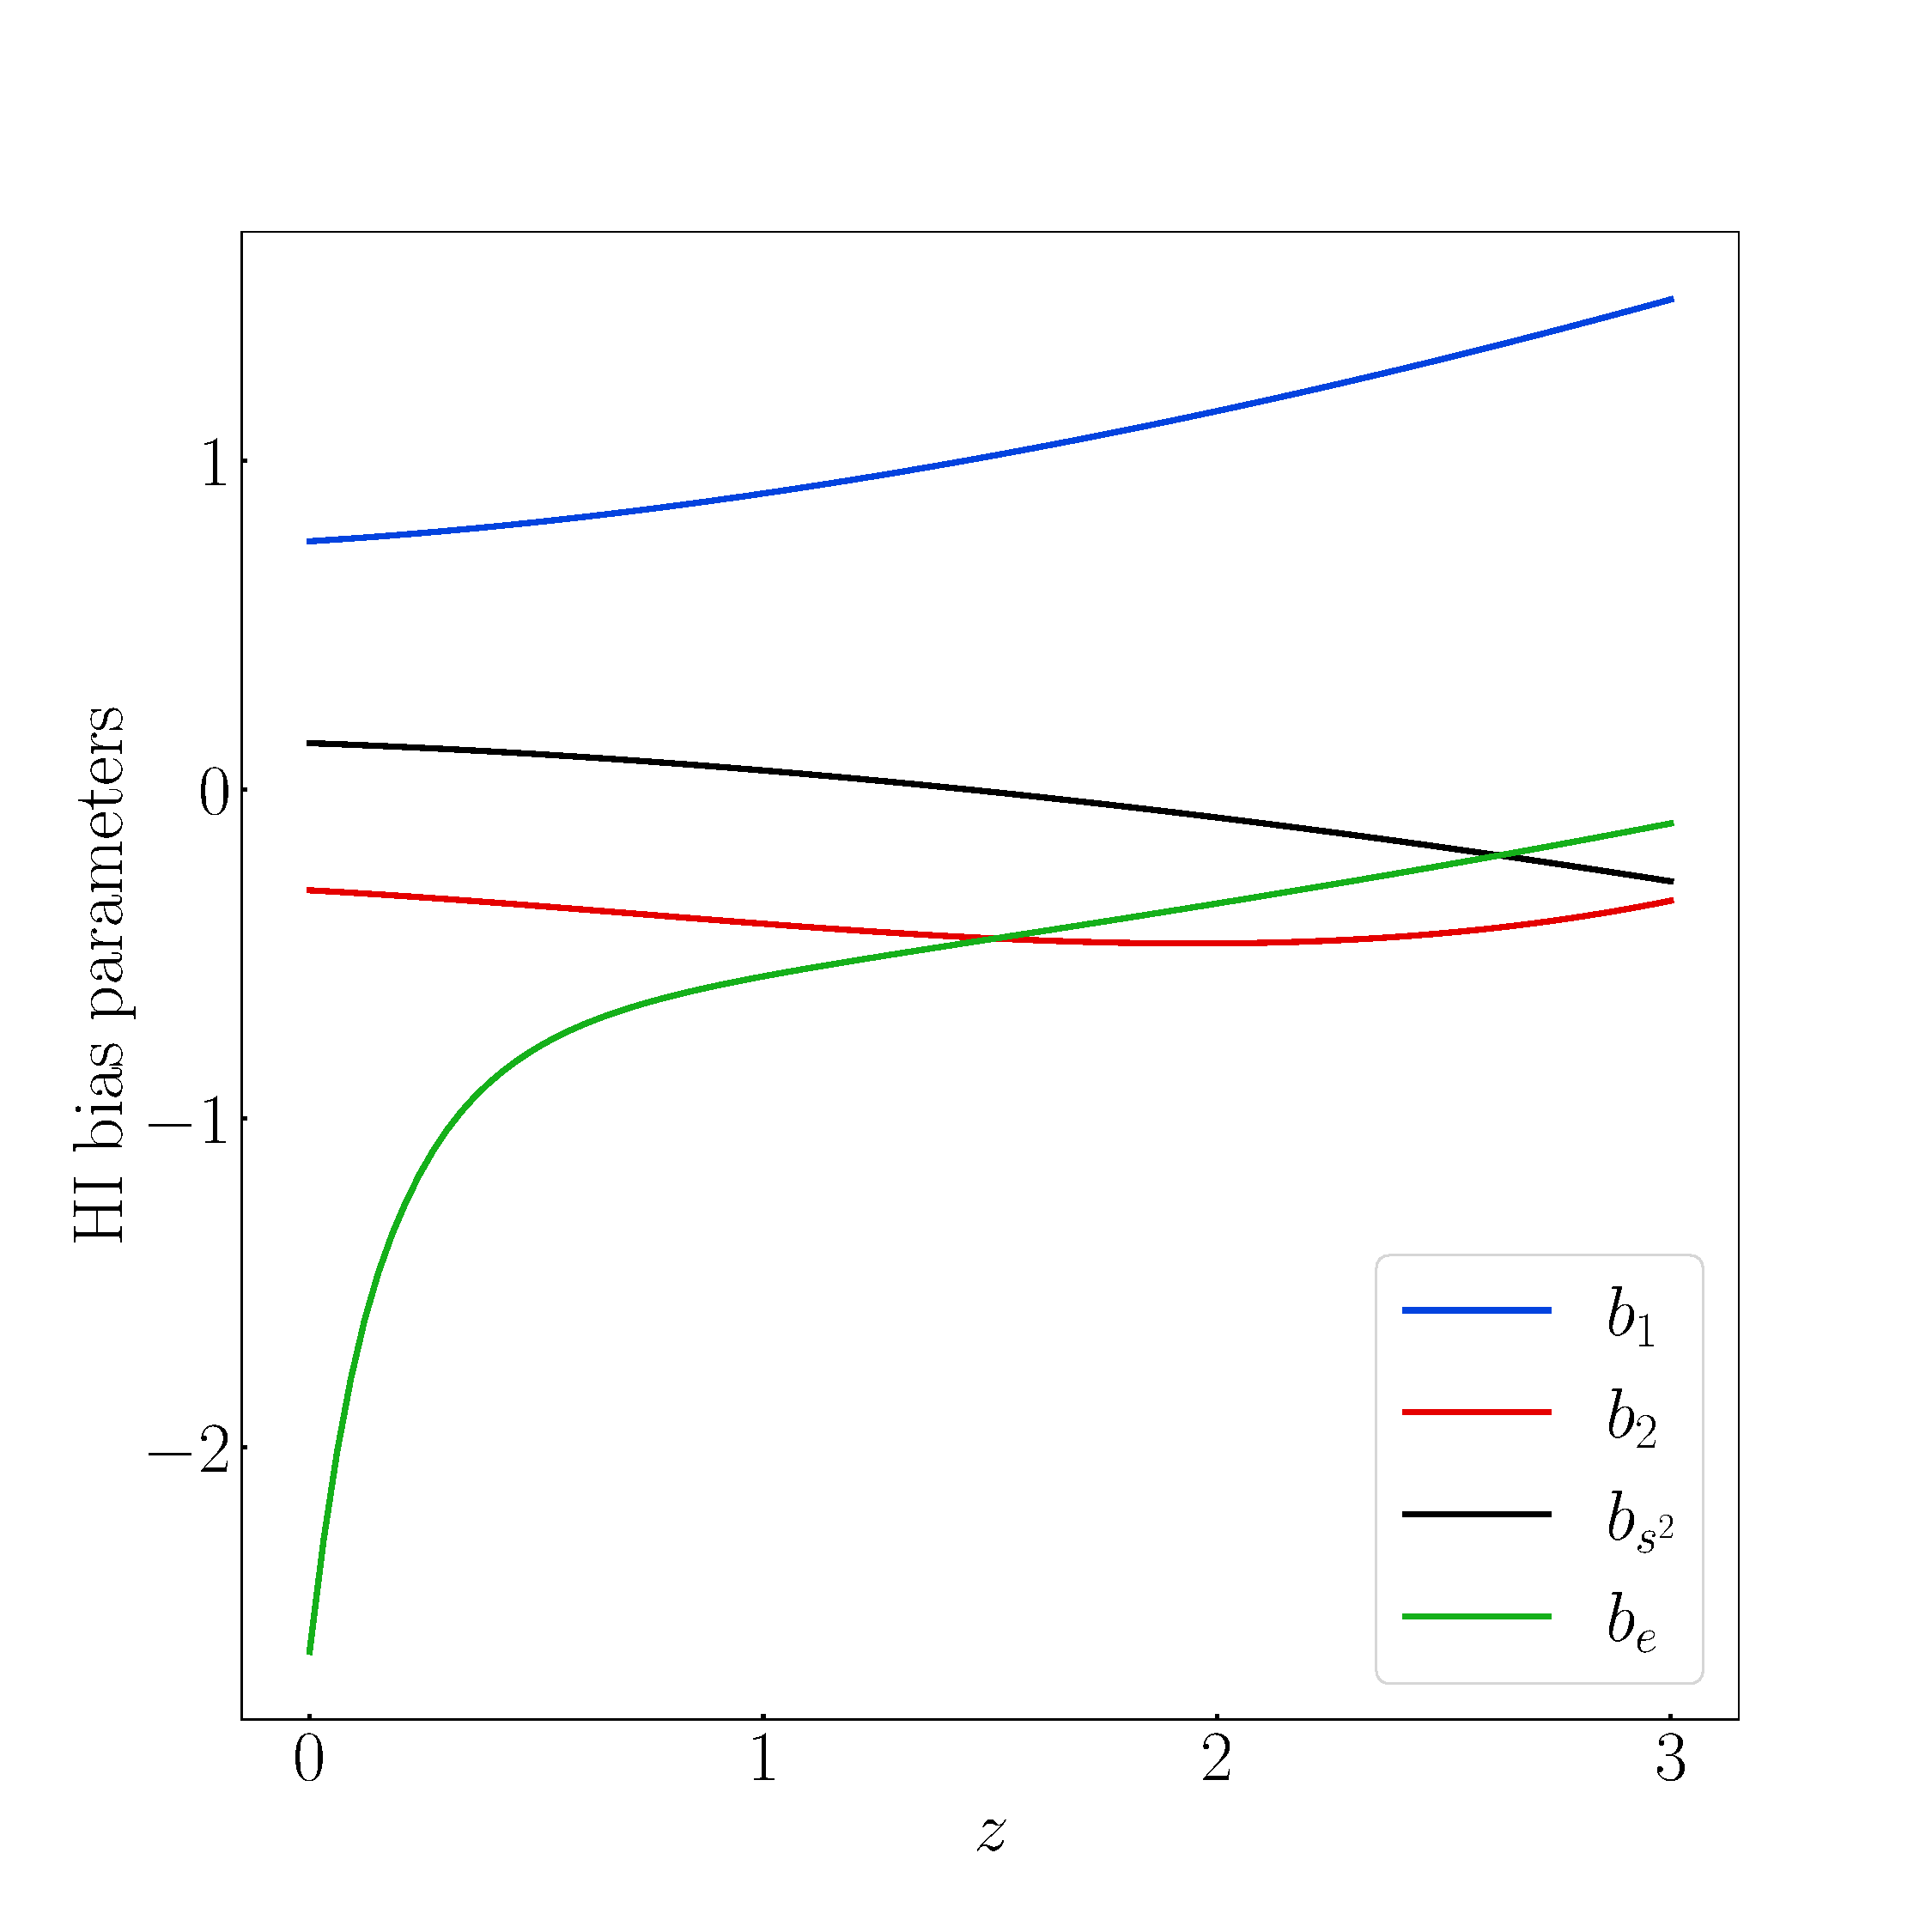
\includegraphics[width=.49\textwidth]{fig/HIBias.pdf}
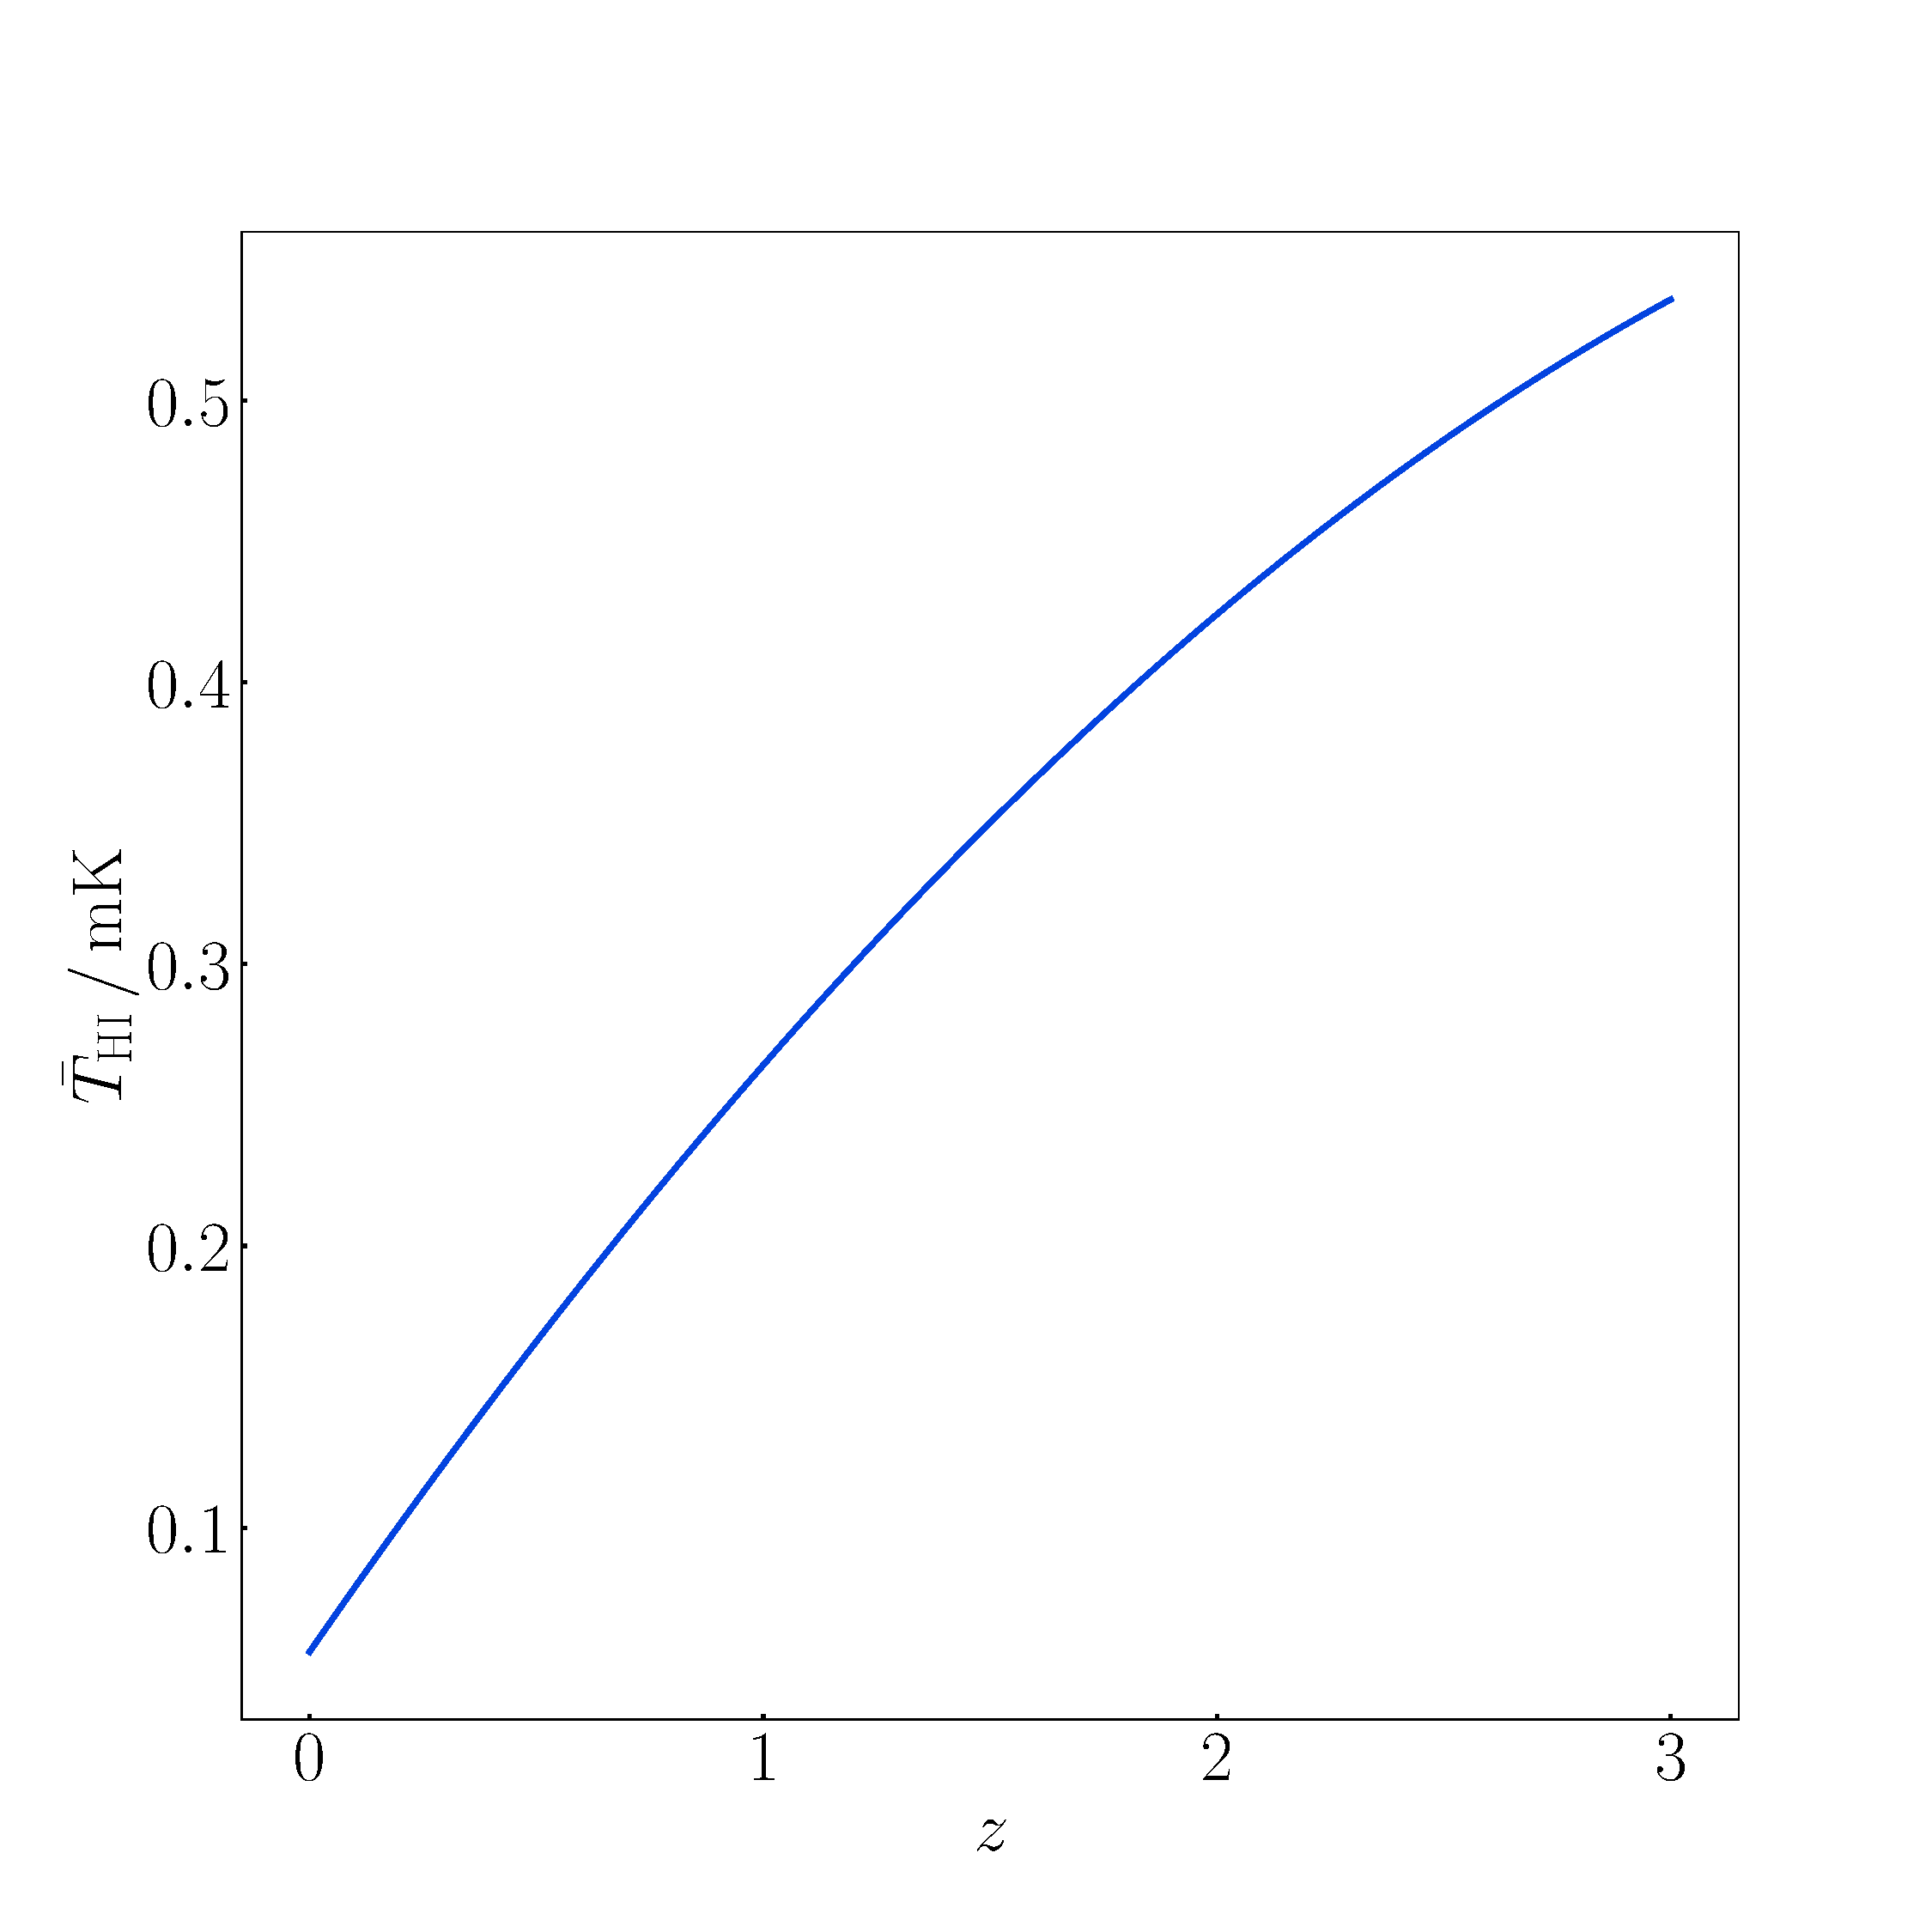
\includegraphics[width=.49\textwidth]{fig/THI.pdf}
%\vspace*{-0.5cm}
\caption{HI clustering and evolution bias parameters (left) and background temperature (right).}\label{fig:detectfigbiasparam}
\end{figure}



\item {\bfseries Lensing contribution:}\\
At first order, there is no lensing contribution to $\Delta$ \cite{Hall:2012wd}. The general case of galaxy number density contrast contains a lensing  contribution $2({\cal Q}-1)\kappa$ to $\Delta_g$, where $\kappa$ is the convergence \cite{Challinor:2011bk}.  For HI emitters in intensity mapping, the magnification bias satisfies
\begin{equation}
{\Q} \equiv -\frac{\p \ln \bar{N}_{\hi}}{\p \ln L}\bigg|_\mathrm{c} = 1\,, \label{magb}
\end{equation}
where c indicates evaluation at the luminosity cut. 

At second order, \eqref{tobs} shows that there is also no contribution to $\Delta^{\tw}$ from lensing convergence \cite{DiDio:2015bua,Jalivand:2018vfz}. We can recover this result from the full general expression for second-order number density contrast  \cite{Bertacca:2014dra, Bertacca:2014wga, Yoo:2014sfa, DiDio:2014lka, Bertacca:2014hwa}, by imposing \eqref{magb} together with the conditions \cite{DiDio:2015bua}
\begin{equation} \label{magb2}
\frac{\p^2 \ln \bar{N}_{\hi}}{\p (\ln L)^2}\bigg|_\mathrm{c} = 0\,, \quad  \frac{\p b_1}{\p \ln L}\bigg|_\mathrm{c}=0\,.
\end{equation}

There remains however a lensing deflection contribution $\nabla_{\perp a}\Delta\,\nabla_\perp^a\phi$ to  $\Delta^{\tw}$,  where $\nabla_{\perp a}$ is a screen-space gradient and $\phi$ is the lensing potential \cite{Umeh:2015gza,DiDio:2015bua,Jalivand:2018vfz}. In the bispectrum the contribution of this term is negligible for equal-redshift correlations \cite{DiDio:2015bua,Durrer:2020orn}. Since we only consider the bispectrum at equal redshifts, we can safely neglect this term. 
\end{itemize}}
\vspace{0.2cm}
\iffalse
In Fourier space, the  HI bispectrum  at  tree level  is defined by
\begin{equation}
\big\langle \Delta(z,\bm{k}_{1})\Delta(z,\bm{k}_{2})\Delta^{(2)}(z,\bm{k}_{3}) \big\rangle + \text{2 cp}=2 (2\pi)^3 B_{\rm HI}(z, \bm{k}_{1}, \bm{k}_{2}, \bm{k}_{3}) \delta^{\rm Dirac}\big(\bm{k}_{1}+ \bm{k}_{2}+ \bm{k}_{3} \big)\,, \label{e1.3}
\end{equation}
where cp denotes cyclic permutation. It follows that
%and the factor 2 on the right is due to the convention that the total HI brightness contrast is $\Delta^{(1)}_{\rm HI}+ \Delta^{(2)}_{\rm HI}/2$. 
\begin{equation}
B_{\rm HI}(z, \bm{k}_{1}, \bm{k}_{2}, \bm{k}_{3}) = \mathcal{K}^{(1)}(z, \bm{k}_{1})\mathcal{K}^{(1)}(z, \bm{k}_{2})\mathcal{K}^{(2)}(z, \bm{k}_{1}, \bm{k}_{2}, \bm{k}_{3})P_{\rm m} (z, k_{1})P_{\rm m} (z, k_{2}) + \text{2 cp}\;, \label{e1.5}
\end{equation} 
where $P_{\rm m} $ is the linear matter power spectrum (computed using CLASS \cite{Blas:2011rf}).  From now on, we often drop the $z$ dependence for brevity.  
The  bispectrum kernels are as follows.
\begin{itemize}
\item
{\bf Standard (Newtonian) kernels:}
\begin{align}
\mathcal{K}^{(1)}_{\rm N}(\bm{k}_{a}) &= b_{1}+f\mu_{a}^{2}\,,  \label{e1.7} \\ 
\mathcal{K}^{(2)}_{\rm N}(\bm{k}_{1}, \bm{k}_{2},{\bm{k}_3}) &= b_{1}F_{2}(\bm{k}_{1}, \bm{k}_{2}) + b_{2} + f\mu_{3}^{2}G_{2}(\bm{k}_{1}, \bm{k}_{2}) +{fZ_2}(\bm{k}_{1}, \bm{k}_{2})
+ b_{s^{2}}S_{2}(\bm{k}_{1}, \bm{k}_{2})\,, \label{e1.8}
\end{align}
where $f$ is the linear matter growth rate, $\mu_a=\hat{\k}_a\cdot\n$ and the standard $F_2,G_2,Z_2,S_2$ kernels are given in \cite{Maartens:2019yhx}.

\item
{\bf Leading-order relativistic kernels:} 
\begin{align}
\mathcal{K}^{(1)}_{\mathrm{D}}(\bm{k}_{a}) &= \mathrm{i}\,\cH f A\,\frac{\mu_{a}}{k_{a}}\,, \label{e1.9} \\
\mathcal{K}^{(2)}_{\mathrm{D}}(\bm{k}_{1},\bm{k}_{2},\bm{k}_{3}) &= \mathrm{i}\,\cH f \bigg\{
A\,\frac{\mu_{3}}{k_{3}}G_{2}(\bm{k}_{1},\bm{k}_{2})
+{\Big[b_1\big(A+f\big)+{b_1' \over \H} \Big]}\Big(\frac{\mu_{1}}{k_{1}} + \frac{\mu_{2}}{k_{2}}\Big)
\nonumber \\
&  -\frac{3}{2}\Omega_{\rm m} \Big(\mu_{1}^{3}\frac{k_{1}}{k_{2}^{2}} + \mu_{2}^{3}\frac{k_{2}}{k_{1}^{2}}\Big)
+{\Big[\frac{3}{2}\Omega_{\rm m} \big(1+f \big)+2f\big(A-2\big) \Big]}\mu_{1}\mu_{2}\Big(\frac{\mu_{1}}{k_{2}}+\frac{\mu_{2}}{k_{1}}\Big)
\nonumber \\
& +2f\,  {\hat{\bm{k}}_{1} \cdot \hat{\bm{k}}_2}\Big(\frac{\mu_{1}}{k_{1}} + \frac{\mu_{2}}{k_{2}}\Big) 
-\frac{3\Omega_{\rm m} b_1}{2f}\Big(\mu_{1}\frac{k_{1}}{k_{2}^{2}} + \mu_{2}\frac{k_{2}}{k_{1}^{2}}\Big)\!  \bigg\}\,,\label{e1.10}
\end{align}
where $A$ is given by \eqref{eq:AcoeffTrel}. These follow from \eqref{dt1} and \eqref{e1.2}, and {agree with \cite{Maartens:2019yhx} when we impose \eqref{eq:AcoeffTrel}, \eqref{magb} and \eqref{magb2}}.
\item
{\bf Complex bispectrum:}\\
From \eqref{e1.7}--\eqref{e1.10} we see that
$B_{\rm HI}$ is complex: {the imaginary part is given purely by local relativistic corrections, while at leading order, i.e. neglecting relativistic terms of $O(\H^2/k^2)$, the real part is given purely by the standard Newtonian bispectrum:}
\bea
\mathrm{Re}\big(B_{\rm HI}\big) &= &B_{\rm N} = \mathcal{K}^{(1)}_{\rm N}(\bm{k}_{1})\mathcal{K}^{(1)}_{\rm N}(\bm{k}_{2})\mathcal{K}^{(2)}_{\rm N}(\bm{k}_{1}, \bm{k}_{2}, \bm{k}_{3})P_{\rm m} (k_{1})P_{\rm m} (k_{2}) + \text{2 cp}, \label{e1.14}\\
{\mathrm{i \,Im}}\big(B_{\rm HI}\big) &=& B_{\rm D}= \bigg\{\bigg[\mathcal{K}^{(1)}_{\mathrm{N}}(\bm{k}_{1})\mathcal{K}^{(1)}_{\mathrm{D}}(\bm{k}_{2}) + \mathcal{K}^{(1)}_{\mathrm{D}}(\bm{k}_{1})\mathcal{K}^{(1)}_{\mathrm{N}}(\bm{k}_{2})\bigg]\mathcal{K}^{(2)}_{\mathrm{N}}(\bm{k}_{1},\bm{k}_{2},\bm{k}_{3}) 
\label{e1.15}\\ \nonumber 
&&{}~~~~~~~~~~~~~ +\mathcal{K}^{(1)}_{\mathrm{N}}(\bm{k}_{1})\mathcal{K}^{(1)}_{\mathrm{N}}(\bm{k}_{2})\mathcal{K}^{(2)}_{\mathrm{D}}(\bm{k}_{1},\bm{k}_{2},\bm{k}_{3})\bigg\}P_{\rm m} (k_{1})P_{\rm m} (k_{2})+\text{2 cp}.
\eea
It is apparent that {$B_{\rm N} \sim P_{\rm m} ^2$ while $B_{\rm D} \sim {\rm i}\, (\H/k) P_{\rm m} ^2$.}
Equation \eqref{e1.15} makes explicit the coupling of relativistic  and Newtonian terms in the bispectrum.
\end{itemize}
\fi

\subsection{Effects of foregrounds}


\subsection{Maximum and minimum scales probed}
%

\subsection{Instrumental noise}\label{ssec:inoise}


\subsection{Future 21cm IM surveys}

\subsection{Forecasts for single-dish mode experiments}

\subsection{Forecasts for interferometer mode experiments}

\subsubsection{Reducing the radial foreground cut}
